\documentclass[sigconf]{acmart}

\usepackage{booktabs}
\usepackage{balance}
\usepackage{graphicx,lipsum}
\usepackage{fancyvrb}
\graphicspath{ {./images/} }

\acmConference[SPLC'22]{26th International Systems and Software Product Line Conference}{12--16 September, 2022}{Graz, Austria}

\begin{document}

\title{In Three Steps to Software Product Lines: a Practical Example from the Automotive Industry}

\author{Matthias Eggert}
\affiliation{%
    \department{Rhine-Main-Team (RMT)}
    \institution{Marquardt GmbH}
    \streetaddress{Schloss-Str. 16}
    \postcode{78604}
    \city{Rietheim-Weilheim}
    \country{Germany}
}
\email{matthias.eggert@marquardt.com}
\author{Karsten Günther}
\affiliation{%
    \department{Rhine-Main-Team (RMT)}
    \institution{Marquardt GmbH}
    \streetaddress{Schloss-Str. 16}
    \postcode{78604}
    \city{Rietheim-Weilheim}
    \country{Germany}
}
\email{karsten.guenther@marquardt.com}
\author{Jochen Maletschek}
\affiliation{%
    \department{Rhine-Main-Team (RMT)}
    \institution{Marquardt GmbH}
    \streetaddress{Schloss-Str. 16}
    \postcode{78604}
    \city{Rietheim-Weilheim}
    \country{Germany}
}
\email{jochen.maletschek@marquardt.com}
\author{Alexandru Maxiniuc}
\affiliation{%
    \department{Rhine-Main-Team (RMT)}
    \institution{Marquardt GmbH}
    \streetaddress{Schloss-Str. 16}
    \postcode{78604}
    \city{Rietheim-Weilheim}
    \country{Germany}
}
\email{alexandru.maxiniuc@marquardt.com}
\author{Alexander Mann-Wahrenberg}
\affiliation{%
    \department{Rhine-Main-Team (RMT)}
    \institution{Marquardt GmbH}
    \streetaddress{Schloss-Str. 16}
    \postcode{78604}
    \city{Rietheim-Weilheim}
    \country{Germany}
}
\email{alexander.mann-wahrenberg@marquardt.com}

\newpage

\begin{abstract}
    In the automotive industry, suppliers aim to increase their revenue and try
    to keep up with the pace of the market trends to stay competitive by
    offering off-the-shelf products to car manufacturers. On the other hand
    those car manufacturers request tailored products to gain unique selling
    points. Each new customer request may result in a new software project. To
    save time one might find it a good idea to create the new software project
    as a copy of an older one. This method guarantees initial functionality, but
    prevents refactoring and leads to continuous software erosion. The
    implementations diverge from each other and improvements cannot be shared.
    Software Product Lines (SPL) can help to maximize reusability and quality by
    building up shared core assets and customer-specific functionality. In our
    paper, we propose a method to migrate a customer project landscape into a
    scalable SPL in three steps.
\end{abstract}

\begin{CCSXML}
 <ccs2012>
    <concept>
        <concept_id>10011007.10011074.10011092.10011096.10011097</concept_id>
        <concept_desc>Software and its engineering~Software product lines</concept_desc>
        <concept_significance>500</concept_significance>
    </concept>
    <concept>
        <concept_id>10011007.10011074.10011092.10011096</concept_id>
        <concept_desc>Software and its engineering~Reusability</concept_desc>
        <concept_significance>500</concept_significance>
    </concept>
    <concept>
        <concept_id>10011007.10011074.10011111.10011113</concept_id>
        <concept_desc>Software and its engineering~Software evolution</concept_desc>
        <concept_significance>300</concept_significance>
    </concept>
    <concept>
        <concept_id>10011007.10011074.10011081.10011082.10011087</concept_id>
        <concept_desc>Software and its engineering~V-model</concept_desc>
        <concept_significance>100</concept_significance>
    </concept>
</ccs2012>
\end{CCSXML}



\ccsdesc[500]{Software and its engineering~Software product lines}
\ccsdesc[500]{Software and its engineering~Reusability}
\ccsdesc[300]{Software and its engineering~Software evolution}
\ccsdesc[100]{Software and its engineering~V-model}

\keywords{Software Product Line, migration, adoption, incremental migration, automotive, functionality reuse, active projects}

\maketitle

%%%%%%%%%%%%%%%%%%%%%%%%%%%%%%%%%%%%%%%%%%%%%%%%%%%%%%%%%%%%%%%%%%
%%% place content here to separate real paper from setup stuff %%%
%%%%%%%%%%%%%%%%%%%%%%%%%%%%%%%%%%%%%%%%%%%%%%%%%%%%%%%%%%%%%%%%%%
\section{Introduction}\label{introduction}

Development of product families rather than individual products is a goal for
many engineering companies. Product Line Engineering (PLE) is a widely used
approach for reaching this goal. It is common and accepted for electronic and
mechanical developments and thus especially important for the automotive
industry that historically comes from this area~\cite{bookssp19X19}. However,
for quite some time the automotive industry is constantly moving its focus
towards the development of software. This development is still ongoing and
becomes more and more complex each year~\cite{ICSE03498}. In order to stay
competitive in the future and to realize a competitive advantage, a fast
adaption to the market and to customer needs is also required for software.
Offering off-the-shelf software products with tailored customer features will
increase the company's revenue. Fortunately PLE has also been applied to
software engineering for many years already in the form of Software Product
Lines (SPL)~\cite{confsplc2000}. An SPL increases reusability~\cite{Clem02a} and
therefore increases quality and decreases development costs of software by
building up shared core assets and customer-specific functionality. With this
reuse in place, a business will be able to do larger scaling. A higher number of
projects will drastically decrease the development costs compared to traditional
engineering methods and the time-to-market will improve due to less development
effort~\cite{confsplcAzanzaMD21}. Thus an SPL is one possible solution to win
against competitors.

But even after years of research, source code migrations to SPL are still
complicated and there are no bullet proof concepts available that are applicable
to actively running projects with tight release plans. Much research has been
done on product line architectures~\cite{Svahnberg1999EPLA,
confsplcTomashchukLJ21} and system engineering~\cite{confsplcSchaferBAKR21},
about feature model migrations~\cite{ncstrlustuttgartfiINPROC200185,
confsplcGrunerBKR20, confsplcDuszynskiDB19, confsplcFritschAR20}, SPL
evolution~\cite{journalssmrQuintonVRBGS21, Svahnberg1999ESPL, Eise02b,
kconfigKernel} and safety aspects~\cite{confsplcWolschke0SAM19} of SPLs. On the
other hand, Hetrick et al.~\cite{confoopslaHetrickKM06} and Abbas et
al.~\cite{confsplcAbbasJLESS20} have written about the overall process, general
benefits and a change of mindset, but not specifically about source code.
Contrary to Rubin et al.~\cite{confsplcRubinCC13}, cloned variants are no option
for us anymore. Krueger~\cite{Krueger2001SMC} reported different migration
strategies more than 20 years ago already: (1) proactive, (2) extractive and (3)
reactive, but no work described a mixture of extractive and reactive migrations,
which we need for existing and upcoming customer projects. Inspired by the work
of Jepsen et al.~\cite{confsplcJepsenDB07} we aim for a strategy with which we
are able to migrate multiple independent repositories to a scalable SPL,
allowing developers and software product managers to proceed with their own pace
and according to the project plan without risking its deadlines and always being
able to do a step backwards if necessary.

In this paper we propose an iterative and incremental migration strategy in
three steps. We structured the paper in the following way:
Section~\ref{challenge} stating the challenges we faced in our projects and
industry to explain our view on the problem and why standard solutions did not
work for us, section~\ref{solution} explaining our three step solution of the
source code migration in detail, presenting infrastructure and build system
ideas and section~\ref{conclusion} presenting our conclusion, an overview on
where we stand right now and giving a forecast on future work.

\section{Challenge}\label{challenge}

Our migration method is supposed to be a generic solution, but our company's
circumstances might have some influence on the ideas that we share in this
paper. This section will explain the challenges we had, both coming from the
products' nature and its industry and also from our corporate processes and
strategies.

The projects that we migrated are in the area of electric cars for premium
automobile manufacturers. The software is written in (Embedded) C and Matlab and
modelled with AUTomotive Open System ARchitecture (AUTOSAR) with C code
generators. These projects must fulfill Automotive Software Process Improvement
and Capability Determination (ASPICE), ISO26262 and other processes, standards
and regulations of the automotive industry during their development phases to
stay competitive and meet legal requirements. A company will less likely get a
new inquiry when the standards and norms are not fulfilled. The standards are
relevant for the entire SPL development and do not only apply for the delivered
software product, but also for supporting processes and tools like the build
system. Additionally, the build system must be able to handle third party source
code deliveries without modifications. One example for this are AUTOSAR
deliveries. The dependency to a delivered AUTOSAR package is not only a
challenge for the toolchain, but also a chance. Due to AUTOSAR's layered
architecture and its interface and component design, it already provides modular
abstraction for separation of concerns, that can help in building SPL core
assets and to maximize functional reuse.

All migrated projects of our SPL base on the same product, a complex sensor
cluster. For historic reasons every (customer) project was managed as a separate
Dimensions repository. Dimensions is a Source Code Management (SCM) system
similar to Revision Control System (RCS) used at the Marquardt GmbH for source
code administration and project documentation. Each individual source code
repository is a self-contained ready-to-build project, including all required
tools and libraries to build the product binaries, like compilers, MSYS and GNU
Make. The C code was validated with Jenkins nightly builds. Those Jenkins
scripts were located in separate repositories, not part of the project's
repository itself. Unit tests were not running with every change of the source
code as part of CI/CD, but were running on demand.

Whenever a new customer project was kicked-off, it also triggered the start of a
new software project. This software project then started as a clone of another
already existing project (`clone-and-own'). This approach had several benefits:
the setup time was short and because a mature project was taken as basis, the
project's software was stable already and debugging and adapting was possible.
There was less work for generic parts and only hardware and customer-specific
modifications were required. However, this approach also caused a lot of
disadvantages. By simply cloning an existing project there was not only a copy
of functionality available in the new project, but also a copy of all its flaws.
Because of a large number of copies a possible refactoring of reused code had to
be merged back and this meant a high effort. If refactoring is never done, this
approach can result in software erosion, as it did in our projects. The software
erosion noticeably led to higher maintenance efforts at the end phase of the
development and brought up errors late during the product lifecycle. For all the
teams working in these projects, with the problems mentioned above, the idea of
migrating to another platform including a new tool chain, not only sounded like
a mammoth task but unrealistic too, having in mind the tightly planned release
schedules.

With our migration to SPL we try to tackle as many as possible of the mentioned
challenges. The migration is only partially done and still ongoing, but we did
not detect major issues so far. At the same time, we managed to:
\begin{itemize}
  \item migrate `clone-and-own' sources to our SPL,
  \item add variant handling capability to the build system,
  \item replace the outdated SCM system by Git and Bitbucket,
  \item introduce a CI/CD system,
  \item introduce a unit test framework as integral part of the development,
  \item automate the setup of the build environment and reduce the repository size drastically,
  \item stay compliant with all rules and norms,
  \item train the team and
  \item still keep release plans.
\end{itemize}

We will not write about all solution aspects in this paper. The focus will be
on the source code migration process and less on the tools, processes and
performed trainings. Our build system implementation is freely available on
Github.com~\cite{GithubSPL}.

\section{Solution}\label{solution}

Our goal with the migration was to switch the mindset from `my project' to `one
of our product variants' by enabling the software teams to collaborate in a
single Git repository and be able to use all variants in a single IDE instance
(in our case Visual Studio Code) to build any target of any product variant.

Our SPL implementation uses Visual Studio Code plus CMake Tools extension as
IDE, CMake and Ninja for building all required targets, Powershell and Python as
build wrapper and CI/CD test runners.

With the help of our SPL implementation we follow a migration strategy that
consists of three consecutive steps as depicted in Figure~\ref{fig:migrationFlow}.

\begin{figure}[htb]
  \centering
  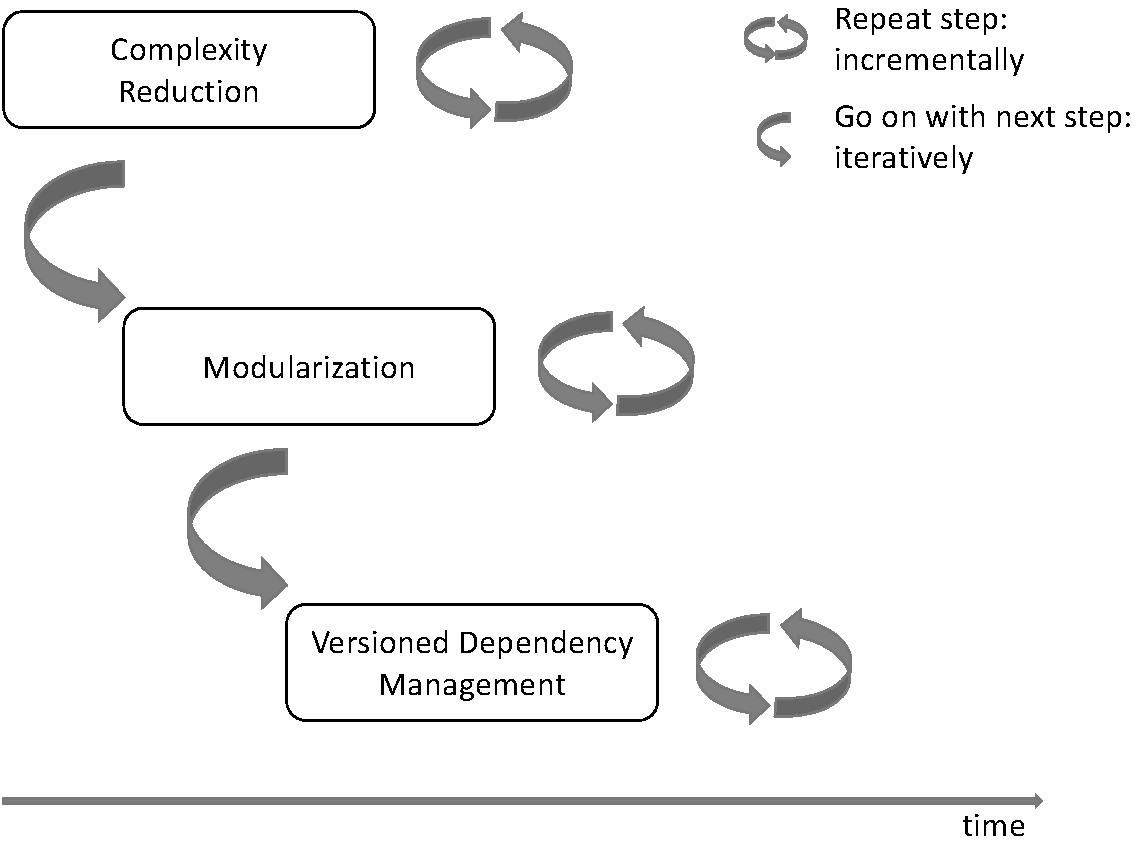
\includegraphics[width=1\columnwidth]{migration-steps-overview.pdf}
  \caption{Migration Flow Overview}
  \Description{Migration Flow Overview showing the three proposed migration steps}
  \label{fig:migrationFlow}
\end{figure}

All three steps will be explained in detail in the following subsections.
It is important to know though, that each step can be done incrementally:
\begin{itemize}
  \item \textit{Complexity Reduction}: variant by variant.
  \item \textit{Modularization}: component by component.
  \item \textit{Versioned Dependency Management}: component by component.
\end{itemize}

If one step is accomplished for a variant or a component, the migration of that
specific variant or component can iteratively proceed with the next migration
step.

The content of the SPL repository, especially the number of lines of code (LOC),
will change during the different migration steps as shown in
Figure~\ref{fig:threeMigrationSteps}. In the first migration step
\textit{Complexity Reduction} the LOC will increase with every legacy project
added to the codebase. During \textit{Modularization} legacy code will be
exchanged with configurable sources leading to a reduction of duplicated code
and therefore to a decreased LOC.\@ Finally even the LOC of configurable sources
in the SPL repository will decrease, as the sources are isolated and moved to a
separate repository during the third step \textit{Versioned Dependency
Management}. Then those configurable sources will just be configured as external
build dependencies in several product families.

\begin{figure*}[ht]
  \centering
  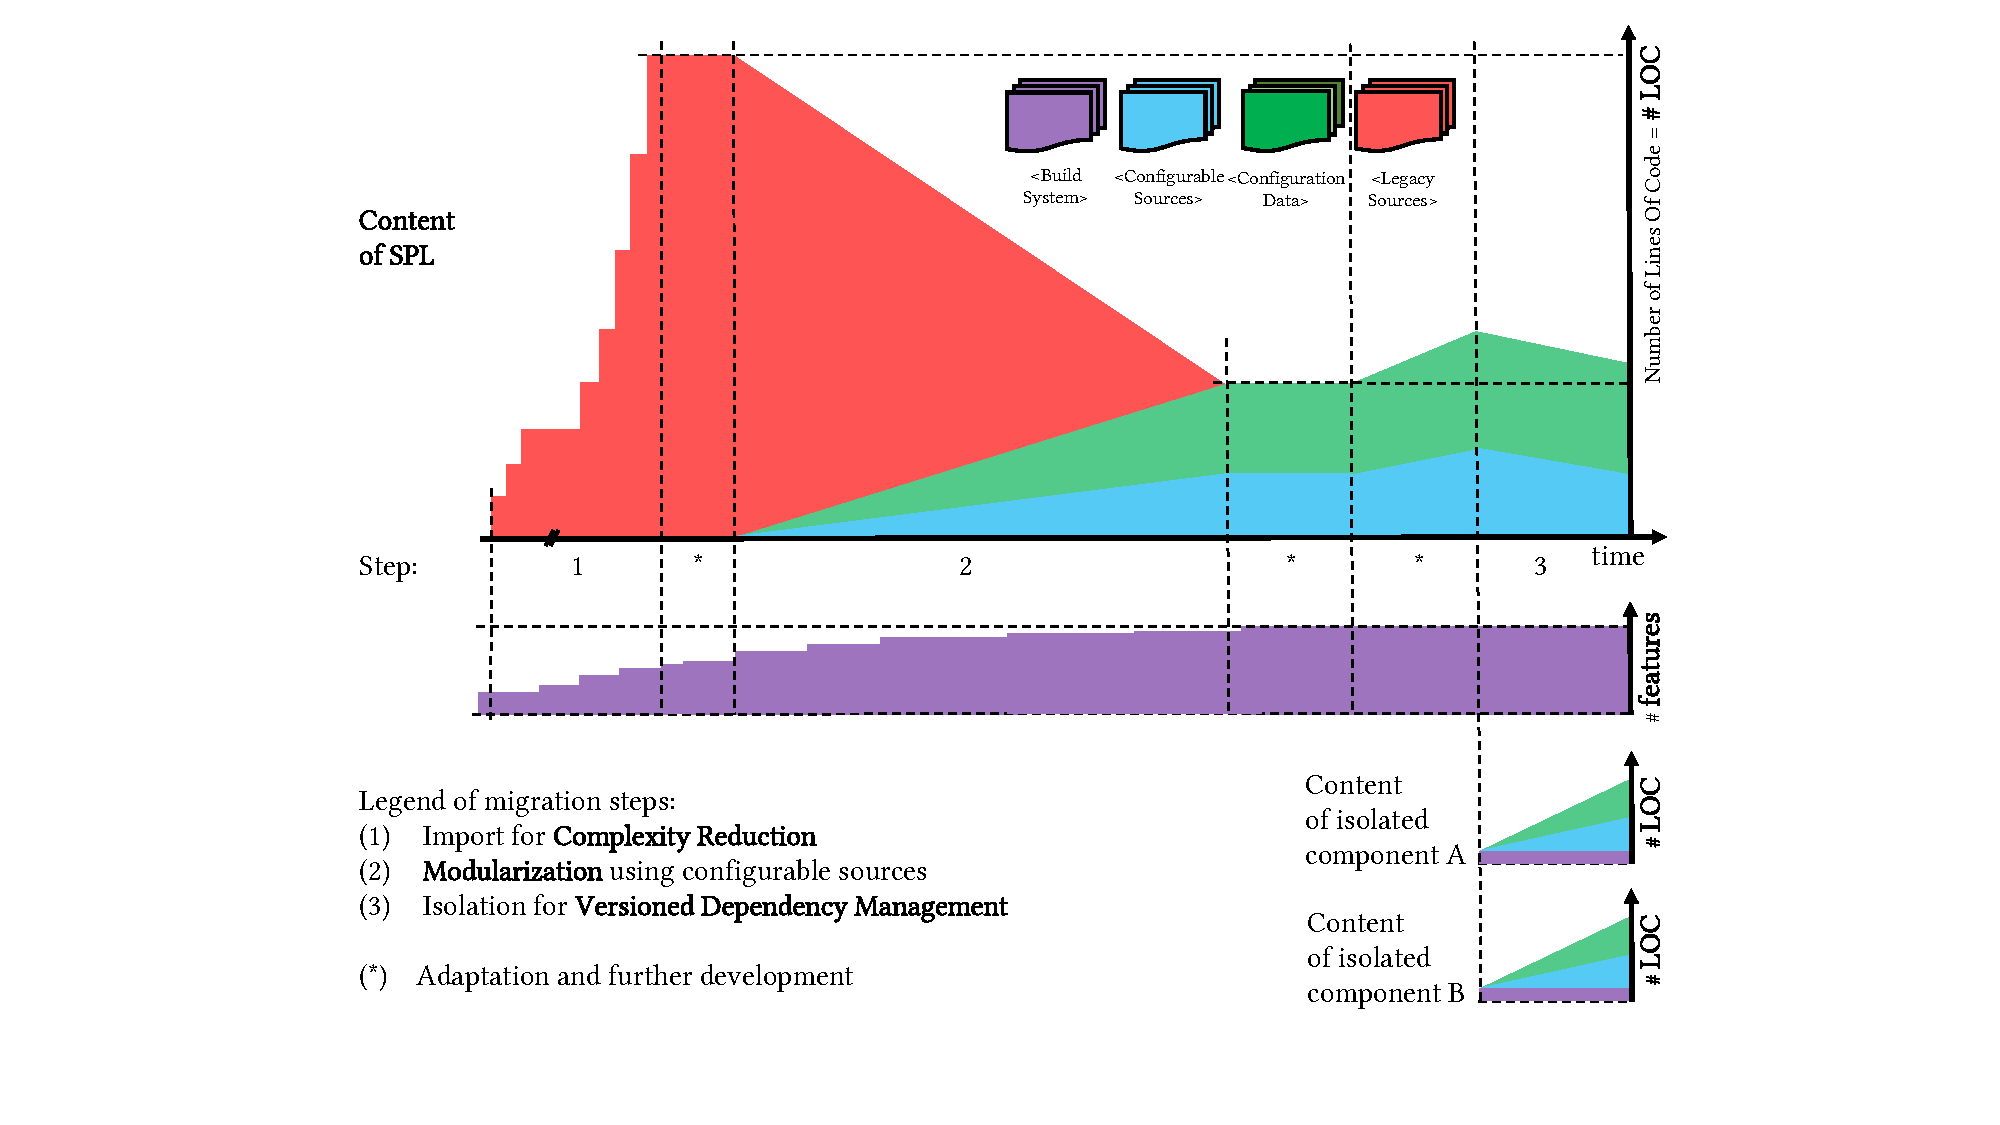
\includegraphics[width=1.55\columnwidth]{migration_steps.pdf}
  \caption{Three Migration Steps to SPL}
  \Description{Three Migration Steps to SPL}
  \label{fig:threeMigrationSteps}
\end{figure*}

\subsection{Complexity Reduction}\label{complexity}

Our first step towards SPL consisted of importing several active sensor projects into
the SPL, i.e., adding Dimension repository product variants into one structured Git
repository. To support further incremental imports of additional sensor variants
we implemented a tool called Transformer~\cite{GithubTransformer} that highly
automates the necessary import steps. The Transformer was implemented in Python
and could be applied to each variant separately, therefore making the transformation
incremental and independent of already existing or upcoming variants. The transformation
of a legacy project into a new product variant is divided into four parts:

\begin{enumerate}
  \item \textbf{Copy sources}: The variant's original source tree is copied
        into a variant-specific legacy tree without any further changes or
        adaptions.
  \item \textbf{Create build configuration}: The original project build
        system (GNU Make) is used to extract all variant-specific configuration and
        to transform it into a CMake configuration and part list compatible with
        the SPL build system.
  \item \textbf{Create IDE configuration}: For seamless integration of the SPL
        repository and its variant concept into Visual Studio Code the
        CMake Tools extension is used. This extension introduces the concept of CMake
        Variants, therefore we create a configuration file with build settings
        for each variant.
  \item \textbf{Establish CI/CD}: In order to simplify the switch to the new
        tool environment, introduce a CI/CD system to increase automation and
        validation for every source code change.
\end{enumerate}

Switching from variant-specific repositories in Dimensions to a single Git
repository in Bitbucket causes a high workflow impact for the developers.
Additionally they need to get used to an SPL build system and a new IDE.\@
Therefore, we decided not to change the production source code during this first
migration step so that the developers can continue to work in their well-known
code basis.

The DevOps Handbook~\cite{devopshandbook} calls this a monolithic approach and
positively emphasizes the simplicity and resource efficiency in small scale. It
also mentions the drawbacks of overall poor scaling and weak modularization
capabilities. We are aware of those drawbacks and are going to tackle them
within the third migration step \textit{Versioned Dependency Management}.

The structure after the transformation looks like this:
\begin{Verbatim}[frame=single,samepage=true]
.vscode/
  cmake-kits.json
  cmake-variants.json
  settings.json
legacy/
  variant-a/
    component-1/
    component-2/
  variant-b/
    component-1/
src/
variants/
  variant-a/
    config.cmake
    parts.cmake
  variant-b/
    config.cmake
    parts.cmake
CMakeLists.txt
\end{Verbatim}

The `legacy' directory contains all the projects' unmodified source code
directories as variant-specific directories. The `src' directory is empty at
first, it will contain the configurable sources. And the `variants' directory
contains the variant configuration in terms of compilation and feature model.

Although the build system and tool environment is reused already for all
variants, for source code there is no reuse in place and the amount of source
code is growing over time as shown in figure \ref{fig:threeMigrationSteps},
therefore scaling may become problematic. Still there are a lot of advantages
with the monolithic way, like centralized deployment with our CI/CD system,
start learning to use Git as source code management system and reducing
complexity by reducing the number of systems: polyrepo vs.\ monorepo with a
single build system and tool environment.

\subsection{Modularization}\label{modularization}

As soon as all developers, software project managers and integrators are used to
the outcome of the first step of the SPL migration, the \textit{Modularization}
step can begin. With the following three stages of \textit{Modularization} it is
possible to switch from a project to a product perspective. Thinking in terms of
products rather than projects helps to reduce the amount of code and maximizes
the reuse across all variants. However, in order to properly build up software
components, consisting of core assets and customer-specific functions, a feature
model definition is required, allowing a configuration of the different software
component characteristics. The goal is to merge the different legacy software
components with similar functionality into configurable sources, keeping
customer-specific functionality, to maximize reuse and reduce maintenance.
Although CMake is capable of handling very simple feature models with variables
and template generators pretty well, a more complex feature model might require
another tool to manage it. Our recommendation for complex feature model
configurations is KConfig, `a domain specific language designed specifically for
coding the Linux kernel variability model'~\cite[page 3]{kconfigKernel}. KConfig
is able to manage the complex design of the Linux kernel and it has enough
functionality to work with most embedded applications. Additionally it is
open-source and free to use for anyone. Alternative solutions might also solve
the configuration purpose. Prominent examples are
pure:variants~\cite{pureVariantsPureSystems} from pure systems or Gears from
BigLever~\cite{gearsBigLever}. Both tools are known to be highly flexible and
easy to integrate into existing projects~\cite{confsplcGrunerBKR20}.

Independent of the feature model tool, the modularization process should be the same.
All stages of the \textit{Modularization} step are visible in
Figure~\ref{fig:step2Modularization} and will be further described in detail:

\begin{figure}
  \centering
  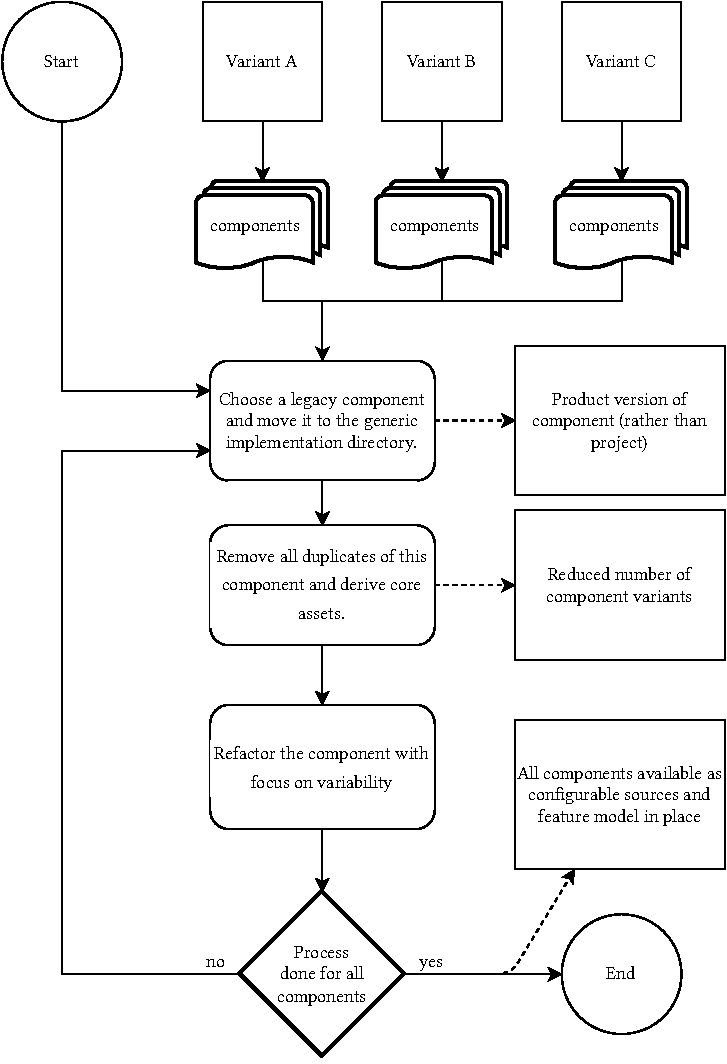
\includegraphics[width=1.0\columnwidth]{step2-modularization-flow.pdf}
  \caption{Detailed stages of the \textit{Modularization} step.}
  \Description{Detailed stages of the Modularization step.}
  \label{fig:step2Modularization}
\end{figure}

\textbf{Migrate from legacy components into product components:} After the first step
\textit{Complexity Reduction}, all source code files are located in a dedicated
legacy directory. This legacy directory contains a folder for each variant,
holding all software components separately. Using a component in multiple
variants is possible, but does not make much sense. There is no reason to share
the variant component variant-a/component-1 also in variant-b. The components do
not belong to a variant, but to the entire product. In this step, components are
just moved into a generic source directory. The folder structure will change
from:
\begin{Verbatim}[frame=single,samepage=true]
legacy/
  variant-a/
    component-1/
    component-2/
  variant-b/
    component-1/
\end{Verbatim}
to:
\begin{Verbatim}[frame=single,samepage=true]
src/
  component-1/
    variant-a/
    variant-b/
  component-2/
    variant-a/
\end{Verbatim}
By doing this, all variants of one component, with the identical or very similar
functionality, are moved to the same directory. Variants of a component residing
next to each other are easier to compare and to handle. This will enable reuse
already, but without the following stages it has no positive effect on source
code reduction or maintenance effort.

\textbf{Remove duplicates and create core assets:} As a first step within this
new structure, we recommend to clean up duplicates. Components are considered as
duplicates if they are identical and no configuration is required. This is a
fast and easy step for reuse and will not require additional knowledge on a
feature model nor on the source code. Removing duplicates is followed by
building up core assets and variant-specific functionality with a decorator
pattern. The separation can be done on a function level. This approach is
enabled by the build system and requires static function interface definitions.
This way the core assets and the decorators can be developed without any need of
conditional compiler directives. The concept is to create a:
\begin{itemize}
  \item core asset C file, which contains generic code across all variants,
        considered to be static,
  \item a header file with interface descriptions of core assets and decorators,
  \item a decorator C file for every variant, which contains a variant-specific
        implementation of a function; the function signature must be identical
        for all variants and shall be defined in the according header file.
\end{itemize}
Like this it is possible to implement variant-specific differences in an
object-oriented manner in C. The idea is to provide a common core asset, which
is meant to stay unchanged, and additionally one interface with multiple
decorators that extend the shared functionality. The feature model's
responsibility is to take control of the underlying build system and configure
the correct decorators. If a separation into core assets and decorators in
individual files is not possible or not useful for any reason, another option
would be to use a feature configuration with conditional preprocessor directives
or runtime configuration. Toggle points in the code make it possible to select
different implementations within the same C file. The feature model's job is to
configure features and control the execution flow.

\textbf{Refactor with focus on variability:} Last but not least, the code should
be refactored according to variability. This is the first refactoring step which
has a functional influence on the code. Previous steps only changed when/how the
source code was compiled. This step is also important because of the mindset
shift. One must stop thinking about project specific features and define
component specific features relevant for the product family. Most of the legacy
components did not support variant handling and some might require substantial
refactorings to have a meaningful feature set.

We highly encourage to implement unit tests before the refactoring starts, if
there are no unit tests available already. During this step the availability of
fast unit tests covering all core assets and features will ensure that no
functionality was broken and will reduce time in finding errors at a later
development phase. Even the non-functional refactorings can have huge affects on
the compiled binaries and change the behavior, even though it was not intended
by the developer. Using features will generate many possibilities to configure
the software. Written unit tests should use the same features to enable/disable
tests or expectations in order to cover all possible execution paths.

\subsection{Versioned Dependency Management}\label{dependencies}

In an SPL we talk about at least two variation dimensions: space,
time~\cite{appliedSPLE} and sometimes also maturity~\cite{bigleverwhitepaper}.
Our first migration step \textit{Complexity Reduction} is merely a step to
prepare these dimensions, to bring code together that belongs together within a
new SPL-capable build system. The second step \textit{Modularization}
establishes the space dimension by building up configurable sources or variants
of software components to reduce lines of code and maximize reuse. With
variation in space we are able to create feature variants of our software and
its components and this is the beginning of the SPL idea. This section will
highlight the time dimension and how the same approach can be used for
cross-product component reuse.

\textbf{Time dimension:} By using Git it is already possible to get a variation
in time. At any created commit, it is possible to create a new branch. This
branch can be the active development branch with all the latest changes, or it
can be based on a former commit to represent a baseline of the SPL that is going
to be released or was released already. If bug fixes are required after a
release happened, they will be done on the same release branch. With this
strategy, releases can be done on a stable code basis without the influence of
new feature developments of other branches. Additionally the documentation of
release relevant changes becomes simple. The release branch will stay unchanged
and usually not get any feature updates, but only fixes. But release branches in
a monorepo come with some drawbacks. It is complicated to get different versions
of different components. A baseline must be done on the entire software. An
integration of mixed versions is possible but requires lots of manual effort and
will likely have a strong negative impact on maintenance. Adding a fix in a
component of a specific version in a release branch will not become available in
the same version of the same component in any other branch. All commits and
branches are independent of each other, so no automatic reuse of code between
them is available. Therefore using the same component and version provides no
reuse in the space dimension if we introduce the time dimension like this. And
finally fixing a bug in a new version, that was spotted in an earlier version,
is even more complicated, especially across all branches. Our proposal requires
some more changes to the build system and infrastructure. It is required to
split up the repository again. With the modularization being done, the split
will not be done per project anymore, but per software component. Each
modularized software component will reside in its own repository and is
maintained separately. This allows us to work with different developers or
development teams on different software components independently. To enable the
development of a software component in its own repository the following
requirements must be fulfilled:
\begin{itemize}
  \item component specific requirements specifications,
  \item mocked required interfaces,
  \item unit tests for all component features in all possible configurations,
  \item software integration tests,
  \item Software-In-the-Loop (SIL) tests and
  \item a software test plan must exist.
\end{itemize}
Although this step introduces a polyrepo workflow it still follows the SPL
concept by dividing products into smaller pieces still developed in SPL
repositories. The SPL repositories of the products do not contain the sources of
the isolated components anymore but each SPL repository has dependencies to
specific versions (baselines) and variants of the isolated components. These
dependencies might be references to commits of a Git repository or to released
component package artifacts, e.g., with JFrog Conan.io. This step can be done
incrementally again, component by component. The SPL repository's build system
will then do the integration job. With a proper dependency management, the build
system will integrate requested software components from external repositories
of any kind and configure them according to the feature model of the selected
variant. The benefits of this approach are the following:
\begin{itemize}
  \item Components are being developed and tested independently to get a faster
        release loop.
  \item A fix of a buggy version is implemented only once in the component's
        repository.
  \item Buggy versions can be marked in the components' repositories. This way
        variant builds containing a buggy version can print a warning or error.
        The integrator can then manually update the version of the dependency or
        justify the warning in regards to their project setup. An automatic
        update would also be possible.
\end{itemize}
Since all components are being developed independently, one package version
might not be compatible with another component's package. With Conan.io
`compatibility can even be configured and customized on a per-package
basis'~\cite{conandocs}. This is why we recommend Conan.io over Git submodules
or similar techniques. The development team together with their integrators can
configure this compatibility check. An AUTOSAR architecture might make this
check easier. An application software component should only have interfaces to
the Run-Time Environment (RTE), so based on the RTE configuration a
compatibility between components should be clearly defined.

\textbf{Cross-product component reuse:} Independent of an SPL introduction, it
is most likely that within the product portfolio of an automotive supplier like
Marquardt with a wide range of different products, those products share similar
components and solutions. When such a company applies SPL engineering for one of
its products, sooner or later the concept is taken over for other products of
other business units, too. In case the second step of SPL migration
\textit{Modularization} is finished in at least two SPL repositories with
similar core assets and step three has been performed on a few components, the
probability, that the need to share those components between the different SPL
repositories will arise, is rather high. Therefore the third step of our
migration concept provides an additional useful feature: isolation of
configurable sources for \textit{Cross-product component reuse}. The idea is
that the isolated software component and all its variants can be used in multiple
other SPL repositories, not just in one. There are functionalities, like current
measurement, that might be useful in a multitude of electronic products. This
can exponentially increase reuse in the entire product portfolio.

\section{Conclusion and Future Work}\label{conclusion}

This work provides an iterative and incremental migration strategy towards SPL
for the software of a real-world product family of an automotive supplier. We
proposed three steps to perform the migration of a project's software repository
to an SPL variant: (1) \textit{Complexity Reduction}, (2)
\textit{Modularization} and (3) \textit{Versioned Dependency Management}. It was
shown that our proposal can be applied to the repositories of a product family's
software at any time of the development phase due to the fact that any of the
three steps can be applied incrementally and each transformed variant can
iteratively continue with the next migration step independent of the others.
With our proposal we:

\begin{itemize}
  \item established a stable SPL with variants buildable at any time,
  \item reduced workload of developers by reducing the number of repositories,
  \item increased collaboration beyond project borders and
  \item integrated all software sources of a product family into one Git
        repository.
\end{itemize}

At the submission date's point of time we managed to proof about 50\% of our
concept. We implemented a build system with modern CMake fully supporting the
concept of SPL variants. The build system prototype required two persons
full-time for six weeks, the implementation for migration step one and two
required two persons full-time for three more months. Over a time frame of two
months we incrementally added ten variants, while each import to the SPL was
really fast due to the automated importing mechanism. We already started with
\textit{Modularization} of software components, but only converted a few
components and begun with removing duplicates. Recently we focussed more on
automation than on the SPL migration, as we saw more advantages there in the
long run. The automation for CI/CD is helpful for the migration as well.

Nevertheless, the build system requires more features, e.g., a package manager
for dependency handling and a unit test framework for Test Driven Development
(TDD) to be able to support our migration steps two and three and we plan to
implement them in the coming months, in parallel to the \textit{Modularization}
of the software components. Additionally it is required to qualify tools which
have an impact on the created binaries or the processes to build them. This tool
qualification is requested by the ISO 26262 standard for safety reasons. We must
take care that CMake, Ninja and KConfig are properly qualified. On the other
hand, proprietary software might come with safety evaluations already. This
should be kept in mind, when deciding for a future tool landscape.

Besides all the discussed technical challenges, there were also social obstacles
on the way to introduce and SPL.\@ Fear of change was probably the strongest
emotion we faced. We feared the introduction of our SPL approach although we
were certain that all required build system features were implemented and we
always had a backup plan to go back to the original repositories. On the other
hand the development team had a lot of doubts to adapt fast enough to new tools
and processes. There was no real threat and still no one had enough confidence
to start the migration. Afterwards we do not see a reason for hesitation, but
sometimes it simply needs someone brave in the team or someone pushing you. Our
conclusion is: Just do it! And if you break it, make sure you can fix it fast!


\balance{}

\bibliographystyle{ACM-Reference-Format}

%%%%%%%%%%%%%%%%%%%%%%%%%%%%%%%%%%%%%%%%%%%%%%%%%%%%%%%%%%%%%%%%%
%%% place references in references.bib for better structuring %%%
%%%%%%%%%%%%%%%%%%%%%%%%%%%%%%%%%%%%%%%%%%%%%%%%%%%%%%%%%%%%%%%%%
\bibliography{references}

\end{document}